
\begin{figure}
\centering
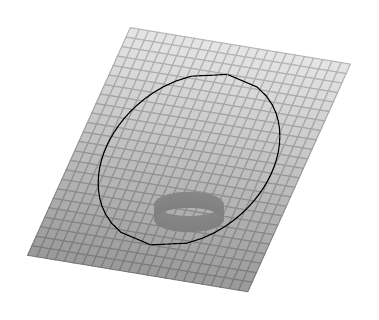
\begin{tikzpicture}[font=\small,declare function={fx(\t)=4-\t;fy(\t)=sqrt(14-(\t-4)^2);fz(\t)=\t;g(\x,\y)=4-\x;hx(\t)=sqrt(2)*cos(\t);hy(\t)=sqrt(2)*sin(\t);hz(\k)=\k;}]
\pgfmathsetmacro{\ta}{4-sqrt(14)}
\pgfmathsetmacro{\tb}{4+sqrt(14)}
\begin{axis}[view/h=115,clip=false,axis lines=center,small,colormap={}{gray(0cm)=(0.6);gray(1cm)=(0.9);},enlargelimits=true,xlabel={$x$},ylabel={$y$},zlabel={$z$},xlabel style={anchor=north},ylabel style={anchor=west},zlabel style={anchor=south},xtick={\empty},ytick={\empty},ztick={\empty},hide axis]
%\addplot3[surf,z buffer=sort,domain=-1:1,domain y=-1:1]{f(x,y)};
\addplot3[surf]({x},{y},{g(x,y)});
\addplot3[surf,domain=0:360,domain y=0:1]({hx(x)},{hy(x)},{hz(y)});
\addplot3[black,domain=\ta:\tb,samples y=1]({fx(x)},{fy(x)},{fz(x)});
\addplot3[black,domain=\ta:\tb,samples y=1]({fx(x)},{-fy(x)},{fz(x)});
\end{axis}
\end{tikzpicture}
\end{figure}



